\chapter{Estado del arte}


La temática del ruido en ambientes urbanos ha marcado todo camino de desarrollo de herramientas tecnológicas con las que se puede observar y tratar este problema desde diversos ángulos (observación de los niveles de contaminación, puntos de mayor presencia de sonidos específicos, sistemas  información, etc). Dichas herramientas implementan diversos métodos que permiten solucionar algún problema en específico de la temática, como por ejemplo la clasificación de sonidos, lo cual se puede lograr por medio de herramientas basadas en Deep Learning. A continuación se dará mención a sistemas y herramientas que buscan hacer frente a la temática o un problema especifico dentro del rango de la misma: 


\section{SONYC}En la ciudad de Nueva York existe una iniciativa para el monitoreo, análisis y mitigación de la contaminación acústica urbana. SONYC consiste en un sistema tipo CPS (cyber-physical system)  el cual se encarga de recolectar datos en forma de audio de distintos lugares de Nueva York para que luego sean procesados para que posteriormente se pueda realizar un análisis de ruido mediante frameworks para la visualización \cite{Bello2018}. En la Figura 6.1 se encuentran los tres elementos claves los cuales se describen a continuación:

\begin{itemize}
\item Recolección de datos (Sensing): los datos se obtienen por medio de dispositivos ubicados en varios lugares de Nueva York y consisten en una Raspberry Pi equipada con un módulo de micrófono de sistemas micro electromecánicos (MEMS). Estos dispositivos generan fragmentos de audio de 10 segundos durante un período de tiempo limitado que posteriormente se comprime con el codificador FLAC, luego se asegura la conexión utilizando AES y RSA. Los nodos se comunican a través de una red privada virtual (VPN)\cite{Bello2018}. 
\item Análisis : El análisis de datos se enfoca en el desarrollo de técnicas de procesamiento de datos e interfaces para la visualización de la información para que pueda ser interpretada tanto de por usuarios con experiencia como aquellos que carecen de ella. Urbane (Figura 6.2) es una de las tecnologías de visualización sobre las que trabaja el grupo de trabajo de SONYC, consiste en un mapa 3D que permite computación en tiempo real, integración y visualización de múltiples flujos de datos\cite{Bello2018}.
\item Actuación: Refiere a técnicas que podrían mitigar. SONYC menciona el efecto de las penalizaciones sobre alguna entidad (empresa o individuo) que de acuerdo al número de ellas puedo reflejar un resultado en cuanto a mitigación a corto y largo plazo. Este análisis de acuerdo con SONYC podría reducir los costos en las intervenciones y aumentar la mitigación del ruido\cite{Bello2018}.
\end{itemize}


\begin{figure}[H]
\centering
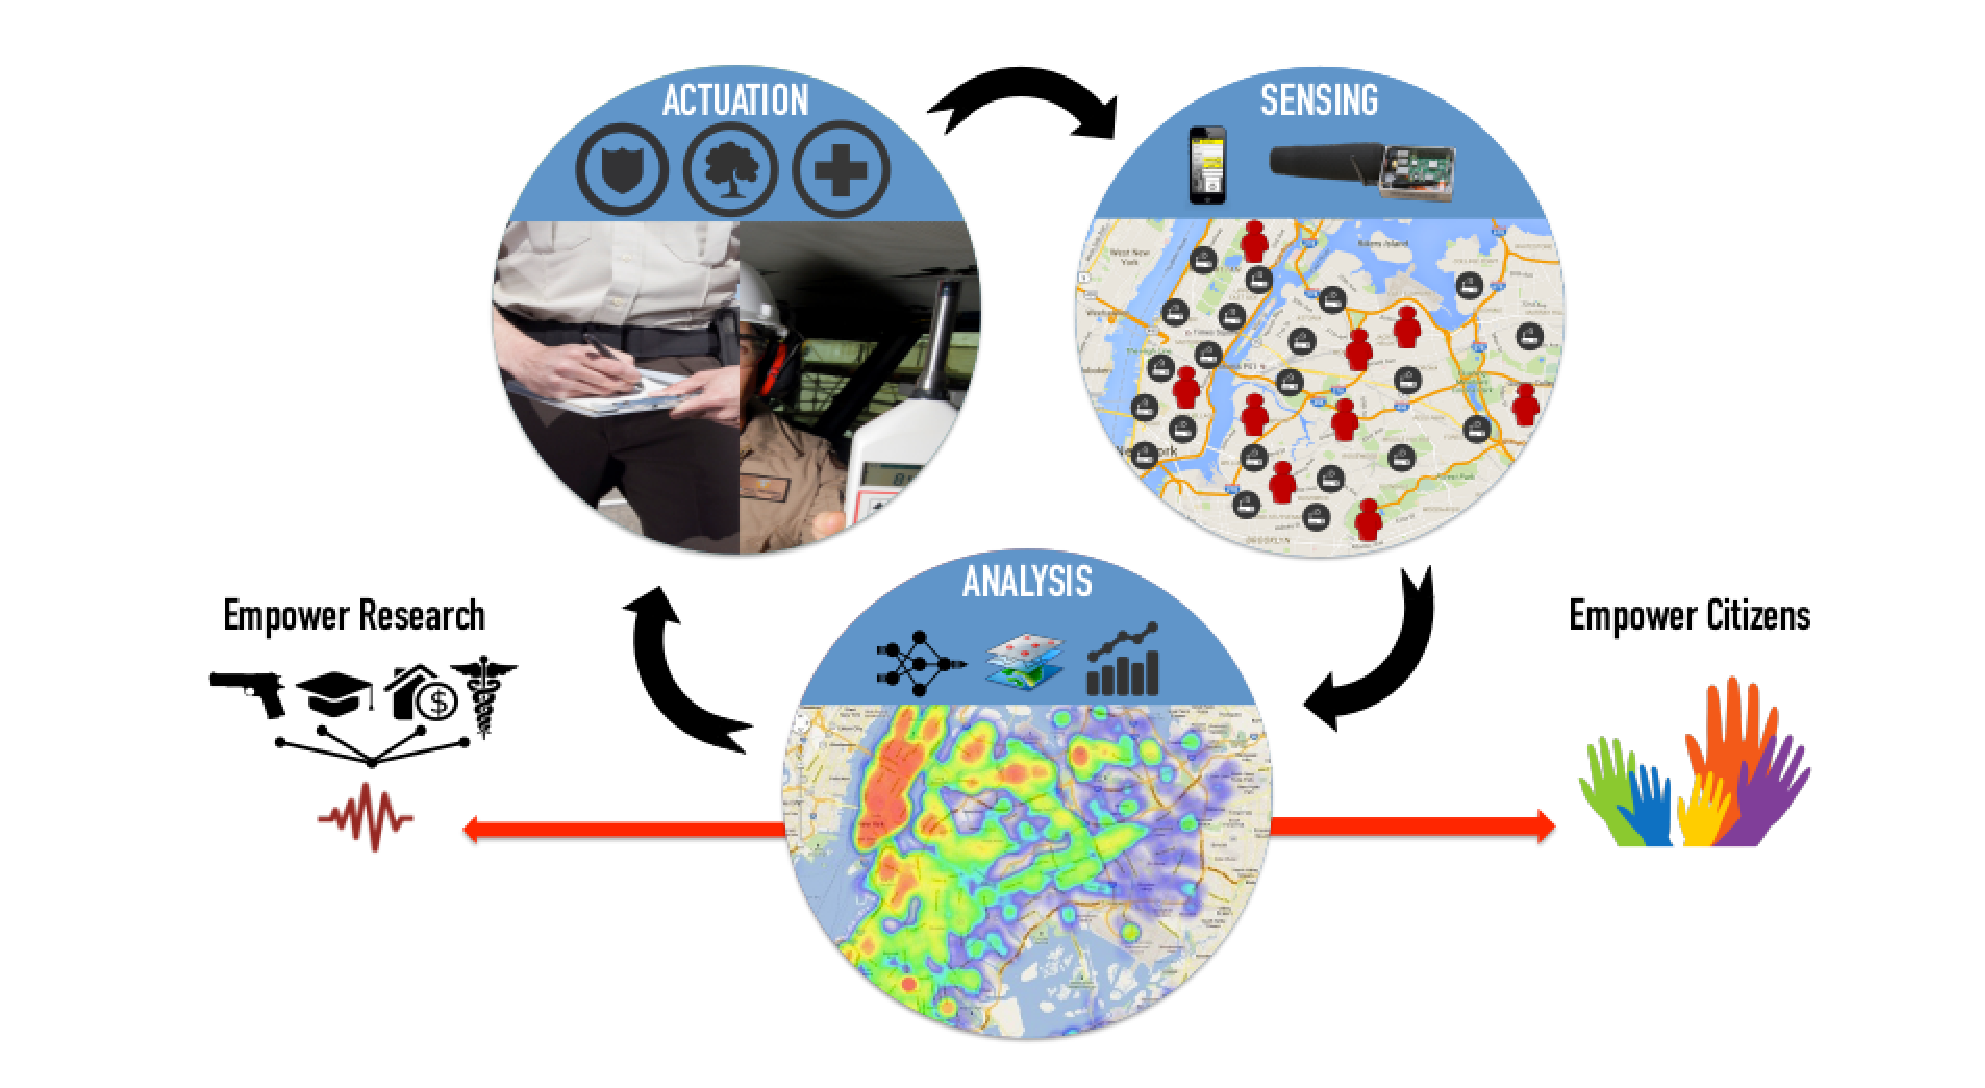
\includegraphics[width=\linewidth]{bibliografia/Imagenes/SONYC.eps}
\caption{SONYC: A System for the Monitoring, Analysis and Mitigation of Urban Noise \cite{Bello2018}}
\end{figure}


\begin{figure}[H]
\centering
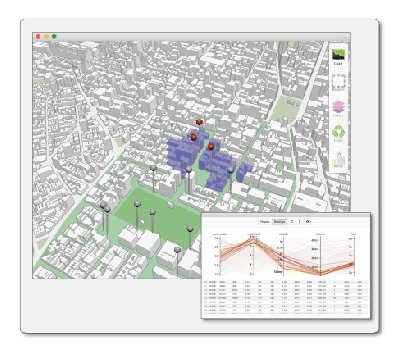
\includegraphics[width=0.6\linewidth]{bibliografia/Imagenes/Urbane.eps}

\caption{Urbane: A 3D framework to support data driven decision making in urban development \cite{Bello2018}}
\end{figure}

\section{Stadtlärm}
Es un sistema de monitoreo de ruido mediante sensores distribuidos (sistemas embebidos) que almacenan y procesan datos en forma de audio, estos son procesados posteriormente en servidores que despliegan servicios para aplicaciones de usuarios. Opera sobre una arquitectura basada en servicio (Broker) utilizando MQTT como protocolo de comunicación \cite{Abeer2019}. Este proyecto como puede observarse en su arquitectura (Figura 6.3) tiene 3 componentes elementales que conforme con el autor se describen a continuación:

\begin{itemize}
    \item Aplicación y visualización: La información es representada en 3D y es usada para diseñar y verificar modelos de ruido-espacio \cite{Abeer2019},\cite{DigitalMediaTechnology2016}.
    \item Unidad de recolección de datos (Acoustic Sensor Units): Se compone de una Raspberry Pi 3, un micrófono MEMS integrado en un PCB y un slot tipo M2 para un módem inalámbrico, y sistemas de protección de agentes externos\cite{Abeer2019}.
    \item Procesamiento de datos (Central Server) : El modelo de clasificación consiste en redes neuronales convolucionales basadas en el modelo de paradigma VGG entrenado para la clasificación entre nueve clases\cite{Abeer2019}.
\end{itemize}

\begin{figure}[H]
\caption{Stadtlärm Project Architecture \cite{Abeer2019} }
\centering
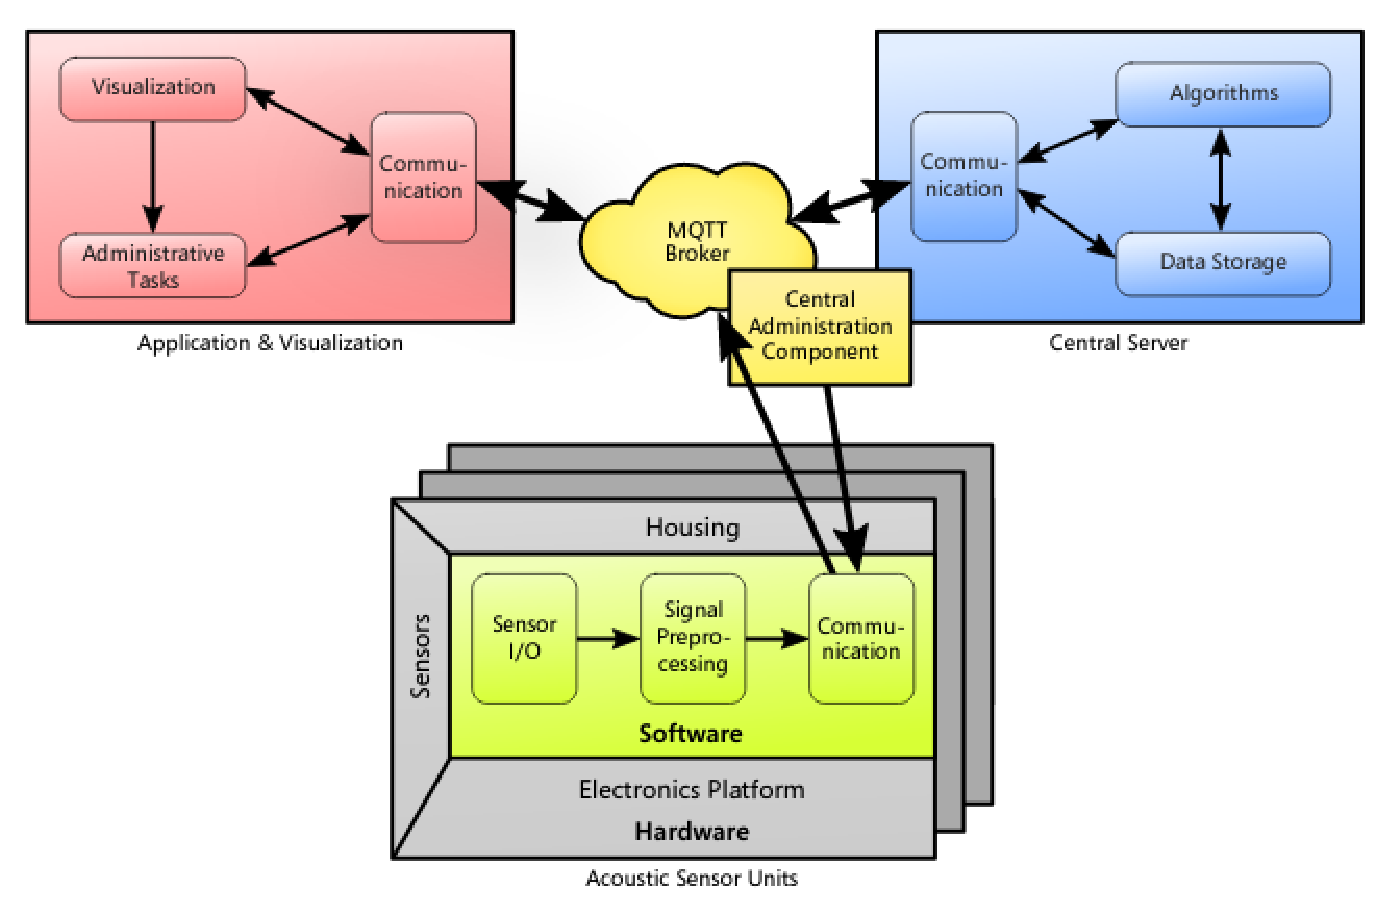
\includegraphics[width=\linewidth]{bibliografia/Imagenes/stadtlarm_arch.eps}
\end{figure}

\section{Dynamap}

Es un proyecto para la actualización de mapas de ruido en tiempo real mediante el uso de mapas básicos de ruido provenientes de diferentes fuentes actualizados mediante una red de sensores de bajo costo en el área de mapeo \cite{Bellucci2018}. Lo mapas básicos son escalonados para proveer un mapa completo del área (Figura 6.4), algunas características se describen a continuación:

\begin{itemize}
    \item Sensores de bajo costo: Existen dos tipos de sensores el primero un sensor de alta capacidad de computo (HCCS) capaz de realizar varias operaciones entre ellas el análisis espectral sobre las señales. El segundo un sensor es de baja capacidad con un limitado número de operaciones y se localiza en los lugares donde no se requiera análisis espectral\cite{Bellucci2018}.
    \item Algoritmo ANED: Es un algoritmo para discriminar sonidos anómalos o aquellos que no sean generados por tránsito rodado. El algoritmo puede identificar entre las siguientes categorías : rodado, ruido de fondo y ruidos anómalos. Los últimos están divididos en 18 categorías\cite{Bellucci2018}.
    \item Aplicación NOISEMOTE : Es un software para la publicación de datos históricos y en tiempo real, se utiliza herramientas estadísticas para mostrar tendencias, valores promedios, entre otros \cite{Bellucci2018}.
    \item web-GIS : Es un software para reescalar mapas básicos de ruido en función de los niveles de ruido detectados por los sensores. Con ellos se genera un mapa completo de un área, los resultado son posteriormente publicados\cite{Bellucci2018}.
\end{itemize}


\begin{figure}[H]
\centering
\includegraphics[width=\linewidth]{bibliografia/Imagenes/dynamap.eps}
\caption{The DYNAMAP project - (Dynamic AcousticMapping - Development of low cost sensors networks for real time noise mapping\cite{Bellucci2018}}
\end{figure}

\section{A Machine Learning Driven IoT Solution for Noise Classification in Smart Cities}

Es un proyecto para la clasificación de ruidos urbanos aplicando IoT y un algoritmo de clasificación basado en SVM (Support Vector Machine) y K-nearest neighbors llegando a una precisión en el rango entre 85\% y 100\%, entrenado utilizando el dataset UrbanSound8K y MFCC (Mel Frequency Cepstral Coefficients) para la extracción de carácteristicas. Como plataforma IoT se utiliza la Raspberry Pi Zero W, un dispositivo de bajo costo y del tamaño de una tarjeta de crédito. Un objetivo de este proyecto es usar edge-computing por lo tanto el algoritmo de clasificación se ejecuta en la plataforma IoT. 

Con base en lo anterior una de las características Edge-computing permiten que el flujo de datos pueda distribuirse hacia puntos cercanos del origen de datos lo cual disminuye la necesidad de realizar el procesamientos de todos los datos en un único centro de datos, añadiendo a esto la capacidad del algoritmo mencionado de ejecutarse en dispositivos de bajo costo con lo cual el dispositivo de procesamiento de datos y origen de datos son el mismo. 